\documentclass{beamer}
\usepackage{tikz}
\usepackage{subcaption}
\usetikzlibrary{calc}
\usepackage{pgfkeys}
\usetikzlibrary{angles, quotes}

\begin{document}
\begin{frame}
\begin{figure}
	\centering
	\begin{subfigure}[t]{0.3\textwidth}
		\centering
		\begin{tikzpicture}[scale=0.75]
			\def\vone{(0.4, 0.4)} % componentes de v1
			\def\vonex{1}
			\def\voney{1}
			
			% ejes
			\draw[gray, -stealth] (-0.2,0) -- (4,0) node[right] {$x$};
			\draw[gray, -stealth] (0,-0.2) -- (0,3.5) node[above] {$y$};
			
			% puntos
			\coordinate (z1) at (3, 1);
			\coordinate (z2) at (1, 2);
			
			\fill (z1) circle (1.5pt) node[below right, font=\footnotesize] {$P$};
			\fill (z2) circle (1.5pt) node[below left, font=\footnotesize] {$Q$};
			
			% vector u en P
			\draw[blue, thick, -stealth] (z1) -- ++(\vonex,\voney) node[midway, right, font=\footnotesize] {$\bf u$};
			
			% vector v en Q: rotación de 60º de u (calculado automáticamente)
			\draw[blue, -stealth] (z2) -- ++({cos(60)*\vonex - sin(60)*\voney}, {sin(60)*\vonex + cos(60)*\voney}) node[midway, right, font=\footnotesize] {$\bf v$};
			

			
		\end{tikzpicture}
		\vspace{-0.3cm}
		\caption{Situación inicial.}
	\end{subfigure}
	\hfill
	\begin{subfigure}[t]{0.3\textwidth}
		\centering
		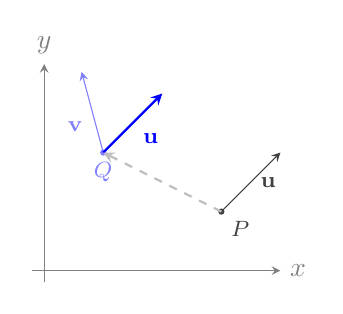
\begin{tikzpicture}[scale=0.75]
			\def\vone{(0.4,0.4)} % componentes de v1
			\def\vonex{1}
			\def\voney{1}
			
			% ejes
			\draw[gray, -stealth] (-0.2,0) -- (4,0) node[right] {$x$};
			\draw[gray, -stealth] (0,-0.2) -- (0,3.5) node[above] {$y$};
			
			% puntos
			\coordinate (z1) at (3, 1);
			\coordinate (z2) at (1, 2);
			
			\fill[darkgray] (z1) circle (1.5pt) node[below right, font=\footnotesize] {$P$};
			\fill[blue!50] (z2) circle (1.5pt) node[below, font=\footnotesize] {$Q$};
			
			% vector u en P
			\draw[darkgray, -stealth] (z1) -- ++(\vonex,\voney) coordinate (puntaV1) node[midway, right, font=\footnotesize] {$\bf u$};
			
			% vector v en Q: rotación de 60º de u 
			\draw[blue!50, -stealth] (z2) -- ++({cos(60)*\vonex - sin(60)*\voney}, {sin(60)*\vonex + cos(60)*\voney}) node[midway, below left, font=\footnotesize] {$\bf v$};
			
			% vector u en Q: paralelo a u, misma norma
			\draw[blue,thick, -stealth] (z2) -- ++({\vonex}, {\voney}) coordinate (puntaV3) node[midway, below right, font=\footnotesize] {$\bf u$};
			
			
			\draw[thick, dashed, -stealth, lightgray] 
			($(z1)!0!(puntaV1)$) 
			--
			($(z2)!0!(puntaV3)$);
			
		\end{tikzpicture}
		\vspace{-0.3cm}
		\caption{Traslación.}
	\end{subfigure}
	\hfill
	\begin{subfigure}[t]{0.3\textwidth}
		\centering
		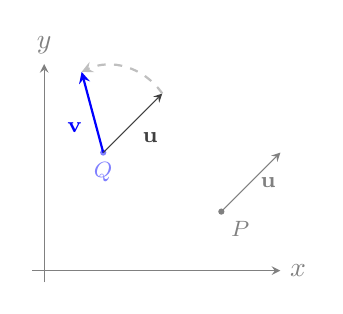
\begin{tikzpicture}[scale=0.75]
			\def\vone{(0.4,0.4)} % componentes de v1
			\def\vonex{1}
			\def\voney{1}
			
			% ejes
			\draw[gray, -stealth] (-0.2,0) -- (4,0) node[right] {$x$};
			\draw[gray, -stealth] (0,-0.2) -- (0,3.5) node[above] {$y$};
			
			% puntos
			\coordinate (z1) at (3, 1);
			\coordinate (z2) at (1, 2);

			
			\fill[gray] (z1) circle (1.5pt) node[below right, font=\footnotesize] {$P$};
			\fill[blue!50] (z2) circle (1.5pt) node[below, font=\footnotesize] {$Q$};
			
			% vector u en P
			\draw[gray, -stealth] (z1) -- ++(\vonex,\voney) node[midway, right, font=\footnotesize] {$\bf u$};
			
			% vector v en Q: rotación de 60º de u 
			\draw[blue, thick, -stealth] (z2) -- ++({cos(60)*\vonex - sin(60)*\voney}, {sin(60)*\vonex + cos(60)*\voney}) coordinate (puntaV2) node[midway, below left, font=\footnotesize] {$\bf v$};
			
			% vector u en Q: paralelo a u, misma norma
			\draw[darkgray, -stealth] (z2) -- ++({\vonex}, {\voney}) coordinate (puntaV3) node[midway, below right, font=\footnotesize] {${\bf u}$};
			
			% flecha curva indicando el movimiento de u a v (sin tocar los vectores)
			\draw[thick, dashed, -stealth, lightgray] 
			($(z1)!1!(puntaV3)$) 
			to[bend right=40] 
			($(z2)!1!(puntaV2)$);


		\end{tikzpicture}
		\vspace{-0.3cm}
		\caption{Rotación.}
	\end{subfigure}
\end{figure}
\end{frame}

\begin{frame}
	\centering
	\begin{figure}
		\centering
		\begin{subfigure}[t]{0.3\textwidth}
			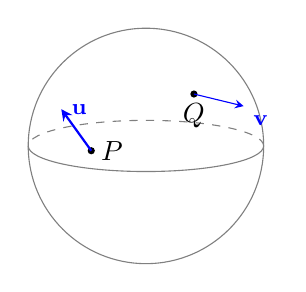
\begin{tikzpicture}[scale=0.65]
					\def\r{2.3}
				\def\h{0.5}
				\def\t{30}
				\def\lat{55}    % ahora es el parámetro phi de Q sobre la elipse (no un radio distinto)
				\def\latp{115}  % parámetro phi de P sobre la elipse
				
				% esfera
				\draw[gray] (0,0) circle (\r cm);
				\draw[dashed, gray] (\r,0) arc[start angle=0,end angle=180,
				x radius=\r cm,y radius=\h cm];
				\draw[gray] (\r,0) arc[start angle=0,end angle=180,
				x radius=\r cm,y radius=-\h cm];
				

				% -------------------------------------------------------
				% P y Q EXACTOS sobre la geodésica: gamma(phi) = R_t * (r cos phi, h sin phi)
				% -------------------------------------------------------
				\pgfmathsetmacro{\Qx}{\r*cos(\lat)*cos(\t) - \h*sin(\lat)*sin(\t)}
				\pgfmathsetmacro{\Qy}{\r*cos(\lat)*sin(\t) + \h*sin(\lat)*cos(\t)}
				\coordinate (Q) at (\Qx,\Qy);
				\fill[black] (Q) circle (2pt) node[below] {$Q$};
				
				\pgfmathsetmacro{\Px}{\r*cos(\latp)*cos(\t) - \h*sin(\latp)*sin(\t)}
				\pgfmathsetmacro{\Py}{\r*cos(\latp)*sin(\t) + \h*sin(\latp)*cos(\t)}
				\coordinate (P) at (\Px,\Py);
				\fill[black] (P) circle (2pt) node[right] {$P$};
				
				% -------------------------------------------------------
				% Tangente EXACTA a la geodésica en P: derivada de gamma(phi), normalizada, rotada t
				% -------------------------------------------------------
				\pgfmathsetmacro{\dPx}{-\r*sin(\latp)}
				\pgfmathsetmacro{\dPy}{\h*cos(\latp)}
				\pgfmathsetmacro{\nPnorm}{sqrt(\dPx*\dPx+\dPy*\dPy)}
				\pgfmathsetmacro{\tx}{(\dPx/\nPnorm)*cos(\t) - (\dPy/\nPnorm)*sin(\t)}
				\pgfmathsetmacro{\ty}{(\dPx/\nPnorm)*sin(\t) + (\dPy/\nPnorm)*cos(\t)}
				\pgfmathsetmacro{\nx}{-\ty}   % normal = tangente rotada 90 grados
				\pgfmathsetmacro{\ny}{\tx}
				
				% Tangente EXACTA a la geodésica en Q
				\pgfmathsetmacro{\dQx}{-\r*sin(\lat)}
				\pgfmathsetmacro{\dQy}{\h*cos(\lat)}
				\pgfmathsetmacro{\nQnorm}{sqrt(\dQx*\dQx+\dQy*\dQy)}
				\pgfmathsetmacro{\tqx}{(\dQx/\nQnorm)*cos(\t) - (\dQy/\nQnorm)*sin(\t)}
				\pgfmathsetmacro{\tqy}{(\dQx/\nQnorm)*sin(\t) + (\dQy/\nQnorm)*cos(\t)}
				\pgfmathsetmacro{\nqx}{-\tqy}
				\pgfmathsetmacro{\nqy}{\tqx}
				
				% -------------------------------------------------------
				% Vector en P
				% -------------------------------------------------------
				\def\ux{cos(270)}
				\def\uy{sin(270)}
				
				\pgfmathsetmacro{\Ux}{\Px + \ux*\tx + \uy*\nx}
				\pgfmathsetmacro{\Uy}{\Py + \ux*\ty + \uy*\ny}
				\coordinate (U) at (\Ux,\Uy);
				\draw[blue, thick, -stealth] (P) -- (U) node[pos=1,right, font=\footnotesize]{$\bf u$};
				
				
				% ---------------------------------
				% Vector v en Q
				% ---------------------------------
				\def\vx{cos(145)}
				\def\vy{sin(145)}
				
				\pgfmathsetmacro{\Vx}{\Qx + \vx*\tqx + \vy*\nqx}
				\pgfmathsetmacro{\Vy}{\Qy + \vx*\tqy + \vy*\nqy}
				\coordinate (V) at (\Vx,\Vy);
				
				\draw[blue, -stealth] (Q) -- (V) node[below right, font=\footnotesize] {$\bf v$};
				
			\end{tikzpicture}
			\caption{Situación inicial.}
		\end{subfigure}
		\hfill
		\begin{subfigure}[t]{0.3\textwidth}
			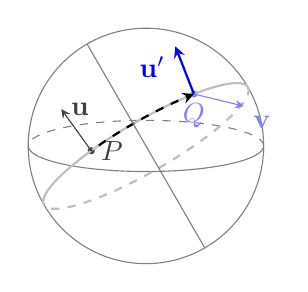
\begin{tikzpicture}[scale=0.65]
				\def\r{2.3}
				\def\h{0.5}
				\def\t{30}
				\def\lat{55}    % ahora es el parámetro phi de Q sobre la elipse (no un radio distinto)
				\def\latp{115}  % parámetro phi de P sobre la elipse
				
				% esfera
				\draw[gray] (0,0) circle (\r cm);
				\draw[dashed, gray] (\r,0) arc[start angle=0,end angle=180,
				x radius=\r cm,y radius=\h cm];
				\draw[gray] (\r,0) arc[start angle=0,end angle=180,
				x radius=\r cm,y radius=-\h cm];
				
				
				
				% -------------------------------------------------------
				% P y Q EXACTOS sobre la geodésica: gamma(phi) = R_t * (r cos phi, h sin phi)
				% -------------------------------------------------------
				\pgfmathsetmacro{\Qx}{\r*cos(\lat)*cos(\t) - \h*sin(\lat)*sin(\t)}
				\pgfmathsetmacro{\Qy}{\r*cos(\lat)*sin(\t) + \h*sin(\lat)*cos(\t)}
				\coordinate (Q) at (\Qx,\Qy);
				\fill[blue!50] (Q) circle (2pt) node[below] {$Q$};
				
				\pgfmathsetmacro{\Px}{\r*cos(\latp)*cos(\t) - \h*sin(\latp)*sin(\t)}
				\pgfmathsetmacro{\Py}{\r*cos(\latp)*sin(\t) + \h*sin(\latp)*cos(\t)}
				\coordinate (P) at (\Px,\Py);
				\fill[darkgray] (P) circle (2pt) node[right] {$P$};
				
				
				% xeodésica
				\draw[lightgray,thick,rotate=\t] (\r,0) arc[start angle=0,end angle=180,
				x radius=\r cm,y radius=\h cm];
				\draw[lightgray, thick,dashed, rotate=\t] (\r,0) arc[start angle=0,end angle=180,
				x radius=\r cm,y radius=-\h cm];
				
				% dibujé la geodésica literalmente, la ploteé
				\draw[dashed,stealth-, black, thick,smooth, domain=\lat:\latp,  variable=\x] plot ({\r*cos(\x)*cos(\t) - \h*sin(\x)*sin(\t)}, {\r*cos(\x)*sin(\t) + \h*sin(\x)*cos(\t)});  
				
				% ------------------------------------
				% recta de giro
				% ------------------------------------
				
				\draw[gray, rotate=\t] (0,\r) -- (0,0);
				\draw[gray, rotate=\t] (0,0) -- (0,-\r);
				
				% -------------------------------------------------------
				% Tangente EXACTA a la geodésica en P: derivada de gamma(phi), normalizada, rotada t
				% -------------------------------------------------------
				\pgfmathsetmacro{\dPx}{-\r*sin(\latp)}
				\pgfmathsetmacro{\dPy}{\h*cos(\latp)}
				\pgfmathsetmacro{\nPnorm}{sqrt(\dPx*\dPx+\dPy*\dPy)}
				\pgfmathsetmacro{\tx}{(\dPx/\nPnorm)*cos(\t) - (\dPy/\nPnorm)*sin(\t)}
				\pgfmathsetmacro{\ty}{(\dPx/\nPnorm)*sin(\t) + (\dPy/\nPnorm)*cos(\t)}
				\pgfmathsetmacro{\nx}{-\ty}   % normal = tangente rotada 90 grados
				\pgfmathsetmacro{\ny}{\tx}
				
				% Tangente EXACTA a la geodésica en Q
				\pgfmathsetmacro{\dQx}{-\r*sin(\lat)}
				\pgfmathsetmacro{\dQy}{\h*cos(\lat)}
				\pgfmathsetmacro{\nQnorm}{sqrt(\dQx*\dQx+\dQy*\dQy)}
				\pgfmathsetmacro{\tqx}{(\dQx/\nQnorm)*cos(\t) - (\dQy/\nQnorm)*sin(\t)}
				\pgfmathsetmacro{\tqy}{(\dQx/\nQnorm)*sin(\t) + (\dQy/\nQnorm)*cos(\t)}
				\pgfmathsetmacro{\nqx}{-\tqy}
				\pgfmathsetmacro{\nqy}{\tqx}
				
				% -------------------------------------------------------
				% Vector en P
				% -------------------------------------------------------
				\def\ux{cos(270)}
				\def\uy{sin(270)}
				
				\pgfmathsetmacro{\Ux}{\Px + \ux*\tx + \uy*\nx}
				\pgfmathsetmacro{\Uy}{\Py + \ux*\ty + \uy*\ny}
				\coordinate (U) at (\Ux,\Uy);
				\draw[darkgray, -stealth] (P) -- (U) node[pos=1,right]{$\bf u$};
				
				% -------------------------------------------------------
				% Transporte paralelo de P a Q: mismas componentes (ux,uy),
				% expresadas en la base local (tangente, normal) EXACTA de Q
				% -------------------------------------------------------
				\pgfmathsetmacro{\Wx}{\Qx + \ux*\tqx + \uy*\nqx}
				\pgfmathsetmacro{\Wy}{\Qy + \ux*\tqy + \uy*\nqy}
				\coordinate (W) at (\Wx,\Wy);
				\draw[blue, thick, -stealth] (Q) -- (W) node[pos=1,below left]{$\bf u^\prime$};
				
				% ---------------------------------
				% Vector v en Q
				% ---------------------------------
				\def\vx{cos(145)}
				\def\vy{sin(145)}
				
				\pgfmathsetmacro{\Vx}{\Qx + \vx*\tqx + \vy*\nqx}
				\pgfmathsetmacro{\Vy}{\Qy + \vx*\tqy + \vy*\nqy}
				\coordinate (V) at (\Vx,\Vy);
				
				\draw[blue!50, -stealth] (Q) -- (V) node[below right] {$\bf v$};
				
				
			\end{tikzpicture}
			\caption{Rotación por geodésica.}
		\end{subfigure}
		\hfill
		\begin{subfigure}[t]{0.3\textwidth}
			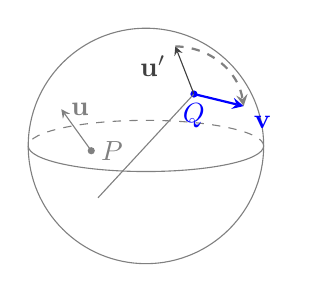
\begin{tikzpicture}[scale=0.65]
				\def\r{2.3}
				\def\h{0.5}
				\def\t{30}
				\def\lat{55}    % ahora es el parámetro phi de Q sobre la elipse (no un radio distinto)
				\def\latp{115}  % parámetro phi de P sobre la elipse
				
				% esfera
				\draw[gray] (0,0) circle (\r cm);
				\draw[dashed, gray] (\r,0) arc[start angle=0,end angle=180,
				x radius=\r cm,y radius=\h cm];
				\draw[gray] (\r,0) arc[start angle=0,end angle=180,
				x radius=\r cm,y radius=-\h cm];
				
				
				
				% -------------------------------------------------------
				% P y Q EXACTOS sobre la geodésica: gamma(phi) = R_t * (r cos phi, h sin phi)
				% -------------------------------------------------------
				\pgfmathsetmacro{\Qx}{\r*cos(\lat)*cos(\t) - \h*sin(\lat)*sin(\t)}
				\pgfmathsetmacro{\Qy}{\r*cos(\lat)*sin(\t) + \h*sin(\lat)*cos(\t)}
				\coordinate (Q) at (\Qx,\Qy);
				\fill[blue] (Q) circle (2pt) node[below] {$Q$};
				
				\pgfmathsetmacro{\Px}{\r*cos(\latp)*cos(\t) - \h*sin(\latp)*sin(\t)}
				\pgfmathsetmacro{\Py}{\r*cos(\latp)*sin(\t) + \h*sin(\latp)*cos(\t)}
				\coordinate (P) at (\Px,\Py);
				\fill[gray] (P) circle (2pt) node[right] {$P$};
				
				\draw[gray] (Q) -- (-\Qx,-\Qy);
				

				% -------------------------------------------------------
				% Tangente EXACTA a la geodésica en P: derivada de gamma(phi), normalizada, rotada t
				% -------------------------------------------------------
				\pgfmathsetmacro{\dPx}{-\r*sin(\latp)}
				\pgfmathsetmacro{\dPy}{\h*cos(\latp)}
				\pgfmathsetmacro{\nPnorm}{sqrt(\dPx*\dPx+\dPy*\dPy)}
				\pgfmathsetmacro{\tx}{(\dPx/\nPnorm)*cos(\t) - (\dPy/\nPnorm)*sin(\t)}
				\pgfmathsetmacro{\ty}{(\dPx/\nPnorm)*sin(\t) + (\dPy/\nPnorm)*cos(\t)}
				\pgfmathsetmacro{\nx}{-\ty}   % normal = tangente rotada 90 grados
				\pgfmathsetmacro{\ny}{\tx}
				
				% Tangente EXACTA a la geodésica en Q
				\pgfmathsetmacro{\dQx}{-\r*sin(\lat)}
				\pgfmathsetmacro{\dQy}{\h*cos(\lat)}
				\pgfmathsetmacro{\nQnorm}{sqrt(\dQx*\dQx+\dQy*\dQy)}
				\pgfmathsetmacro{\tqx}{(\dQx/\nQnorm)*cos(\t) - (\dQy/\nQnorm)*sin(\t)}
				\pgfmathsetmacro{\tqy}{(\dQx/\nQnorm)*sin(\t) + (\dQy/\nQnorm)*cos(\t)}
				\pgfmathsetmacro{\nqx}{-\tqy}
				\pgfmathsetmacro{\nqy}{\tqx}
				
				% -------------------------------------------------------
				% Vector en P
				% -------------------------------------------------------
				\def\ux{cos(270)}
				\def\uy{sin(270)}
				
				\pgfmathsetmacro{\Ux}{\Px + \ux*\tx + \uy*\nx}
				\pgfmathsetmacro{\Uy}{\Py + \ux*\ty + \uy*\ny}
				\coordinate (U) at (\Ux,\Uy);
				\draw[gray, -stealth] (P) -- (U) node[pos=1,right]{$\bf u$};
				
				% -------------------------------------------------------
				% Transporte paralelo de P a Q: mismas componentes (ux,uy),
				% expresadas en la base local (tangente, normal) EXACTA de Q
				% -------------------------------------------------------
				\pgfmathsetmacro{\Wx}{\Qx + \ux*\tqx + \uy*\nqx}
				\pgfmathsetmacro{\Wy}{\Qy + \ux*\tqy + \uy*\nqy}
				\coordinate (W) at (\Wx,\Wy);
				\draw[darkgray, -stealth] (Q) -- (W) node[pos=1,below left]{$\bf u^\prime$};
				
				% ---------------------------------
				% Vector v en Q
				% ---------------------------------
				\def\vx{cos(145)}
				\def\vy{sin(145)}
				
				\pgfmathsetmacro{\Vx}{\Qx + \vx*\tqx + \vy*\nqx}
				\pgfmathsetmacro{\Vy}{\Qy + \vx*\tqy + \vy*\nqy}
				\coordinate (V) at (\Vx,\Vy);
				
				\draw[blue,thick, -stealth] (Q) -- (V) node[below right] {$\bf v$};
				
				
				\draw[gray, thick, dashed, -stealth] (W) to[bend left=40] (V);
				
				
			\end{tikzpicture}
			\caption{Rotación centrada en $Q$.}
		\end{subfigure}
		
	\end{figure}
\end{frame}


\end{document}